\chapter{Background}

\section{Convolutional Neural Networks}



\section{Pose Estimation}
In this work we are heavily inspired by \cite{cao2017realtime} that uses two convolutional neural networks to find human pose. One of the networks finds the probability for the 2D location of a set of joints, we get $N$ confidence maps for the locations of each $N$ number of joints. The other creates $M$ \gls{paf} the probability maps for $M$ number of limbs\footnote{In this work we'll stick to the convention of using the term limb to describe any connection between any pair of body landmarks, which we call joints.}. We then use the results from this \gls{paf} to find out which joints from the first result should be connected.
\begin{figure}[t!]
  \begin{subfigure}[t]{0.24\textwidth}
    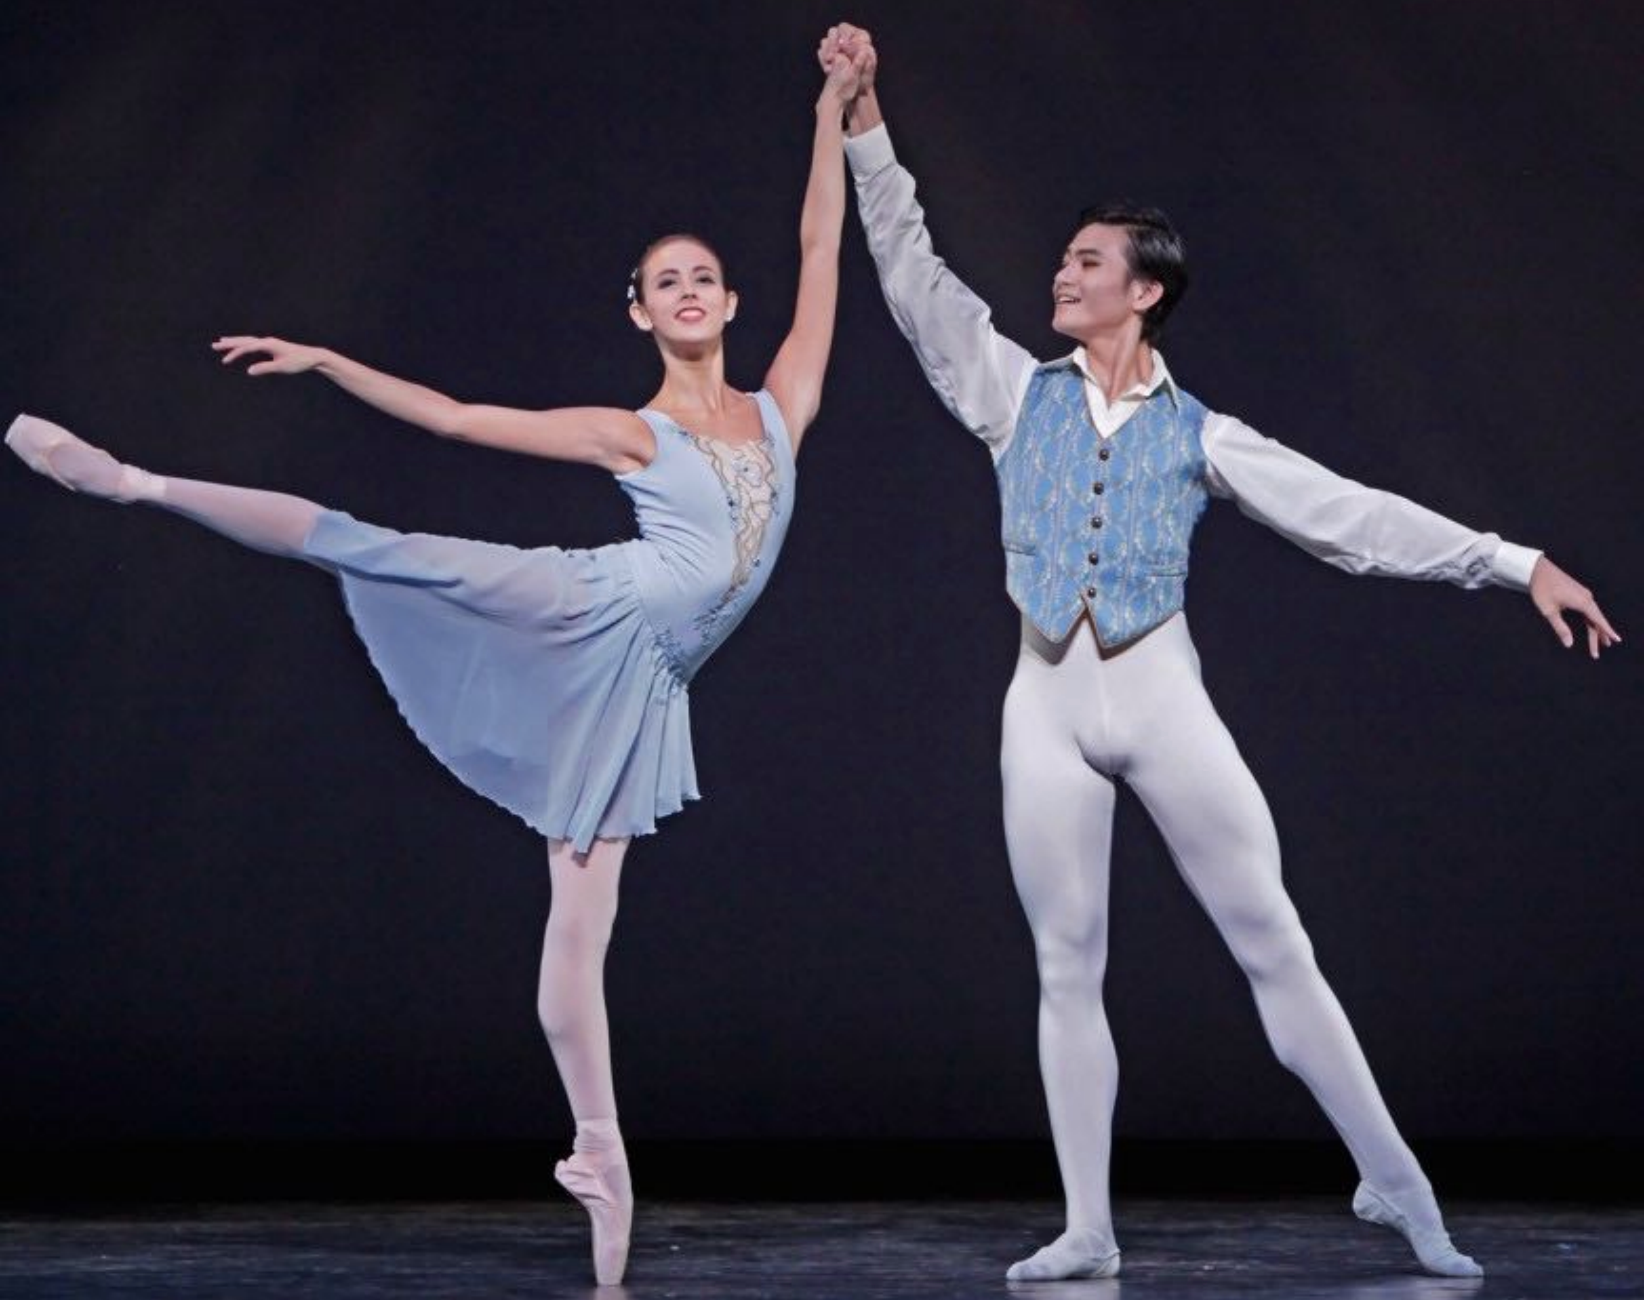
\includegraphics[width=0.9\linewidth]{img/openpose_pipeline_a}
    \label{fig:oppA}
    \caption{Input Image}
  \end{subfigure}%
  ~
  \begin{subfigure}[t]{0.24\textwidth}
    \centering
    \begin{subfigure}[b]{1\textwidth}
      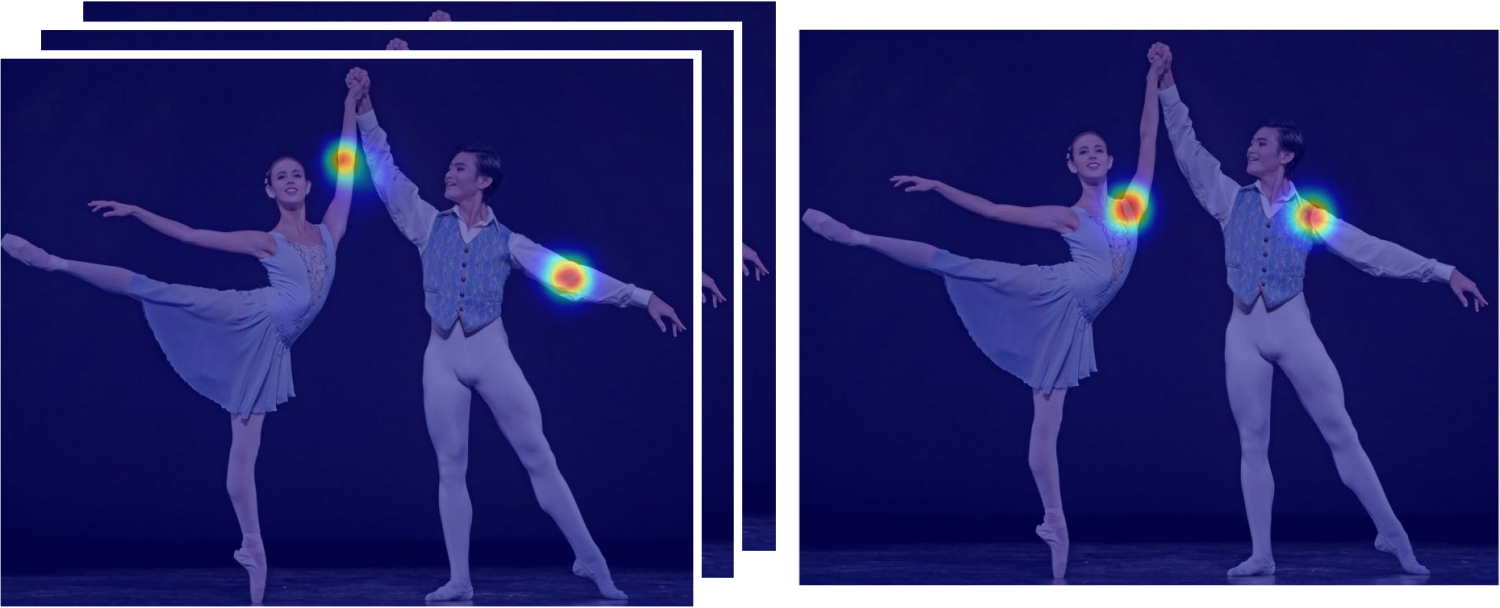
\includegraphics[width=0.9\linewidth]{img/openpose_pipeline_b}
      \label{fig:oppB}
      \caption{Part Confidence Maps}
    \end{subfigure}
    
    \begin{subfigure}[b]{1\textwidth}
      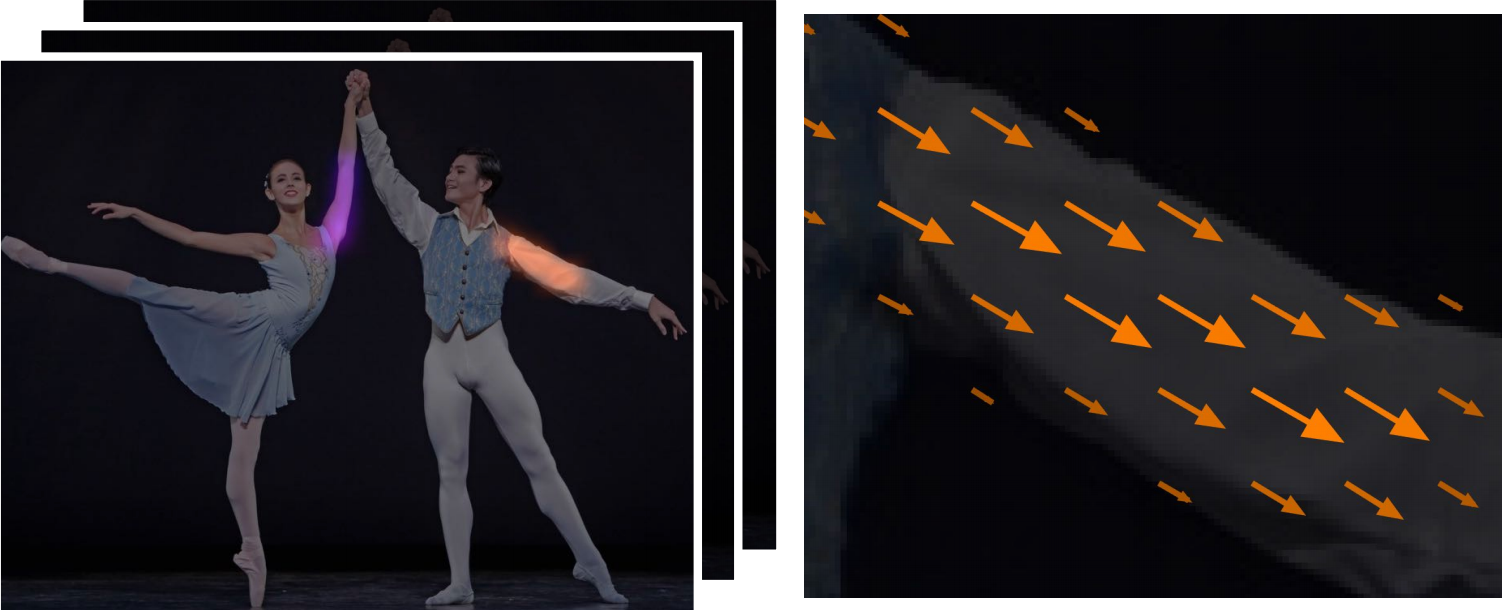
\includegraphics[width=0.9\linewidth]{img/openpose_pipeline_c}
      \label{fig:oppC}
      \caption{Part Affinity Fields}
    \end{subfigure}    
  \end{subfigure}%
  ~
  \begin{subfigure}[t]{0.24\textwidth}
    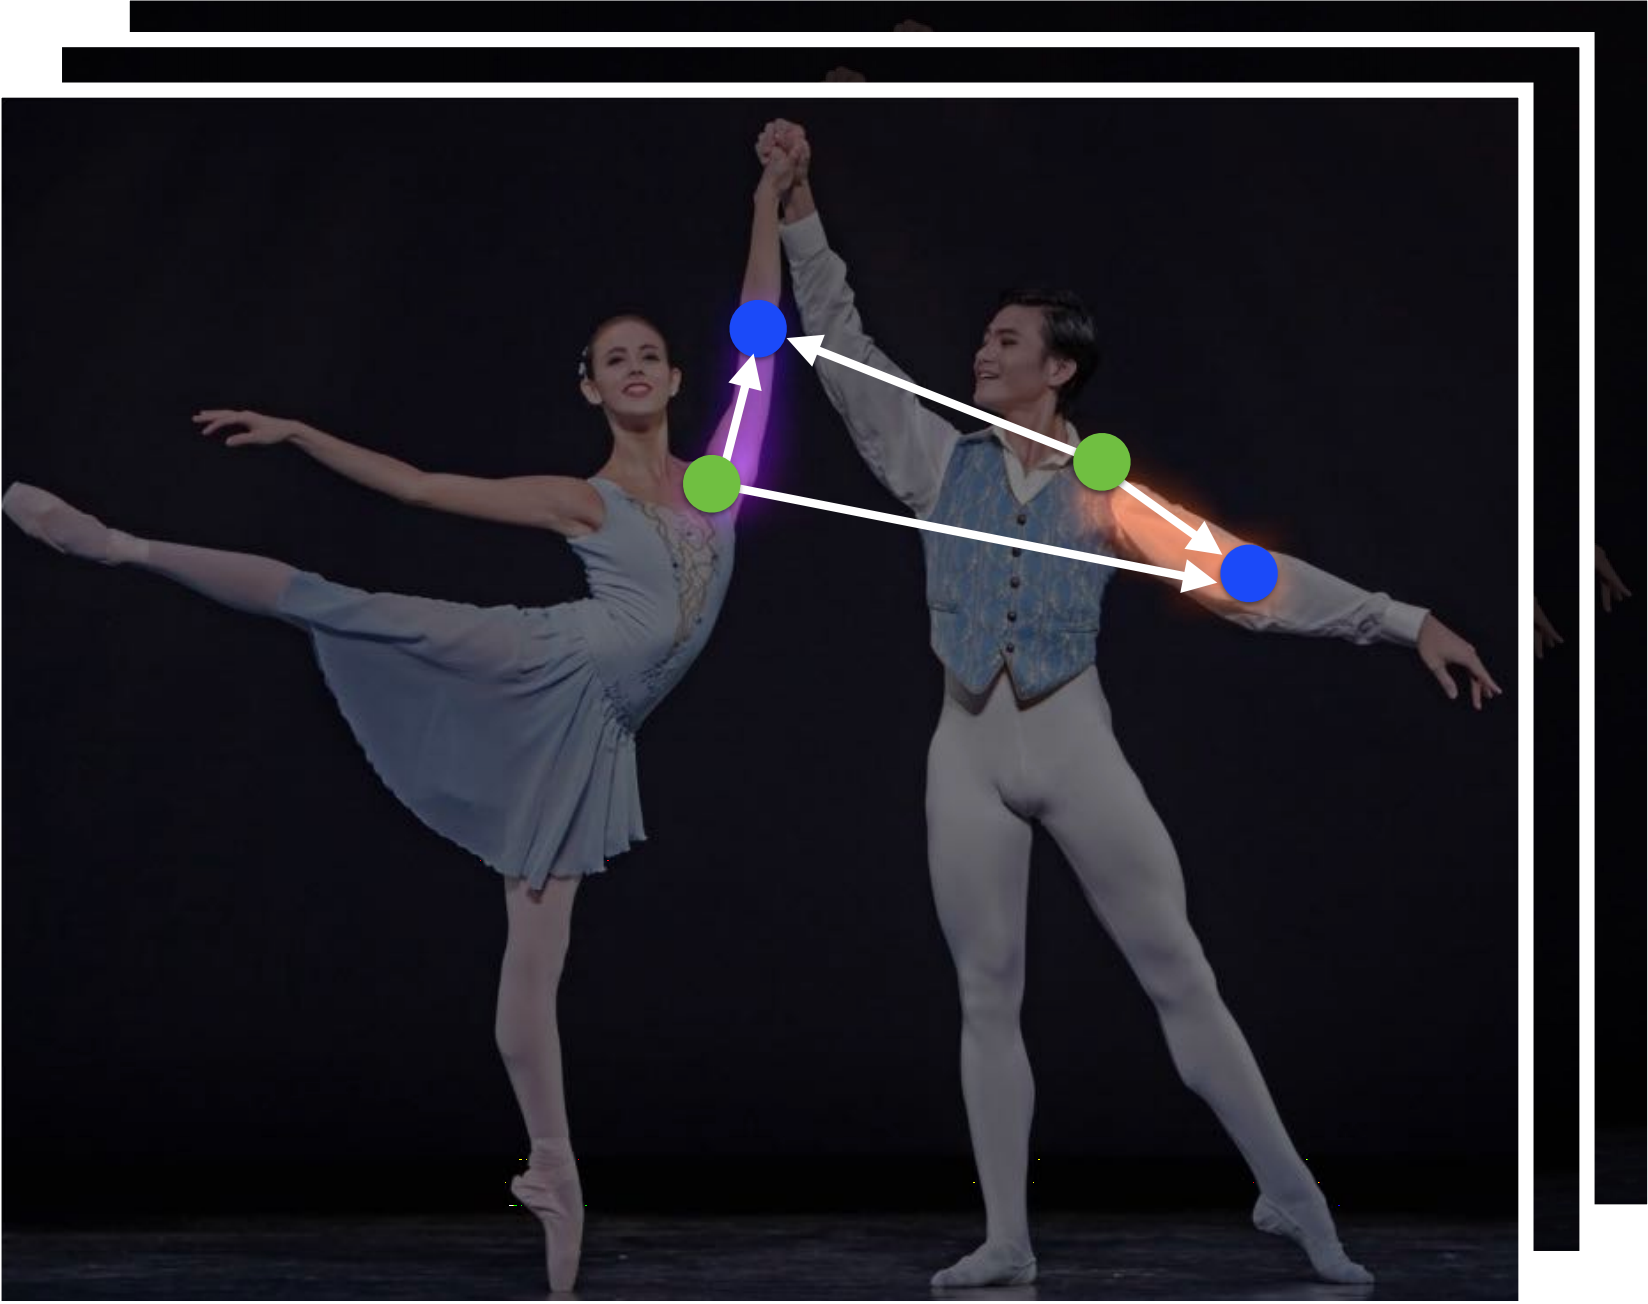
\includegraphics[width=0.9\linewidth]{img/openpose_pipeline_d}
    \label{fig:oppD}
    \caption{Bipartite Matching}
  \end{subfigure}%
  ~
  \begin{subfigure}[t]{0.24\textwidth}
    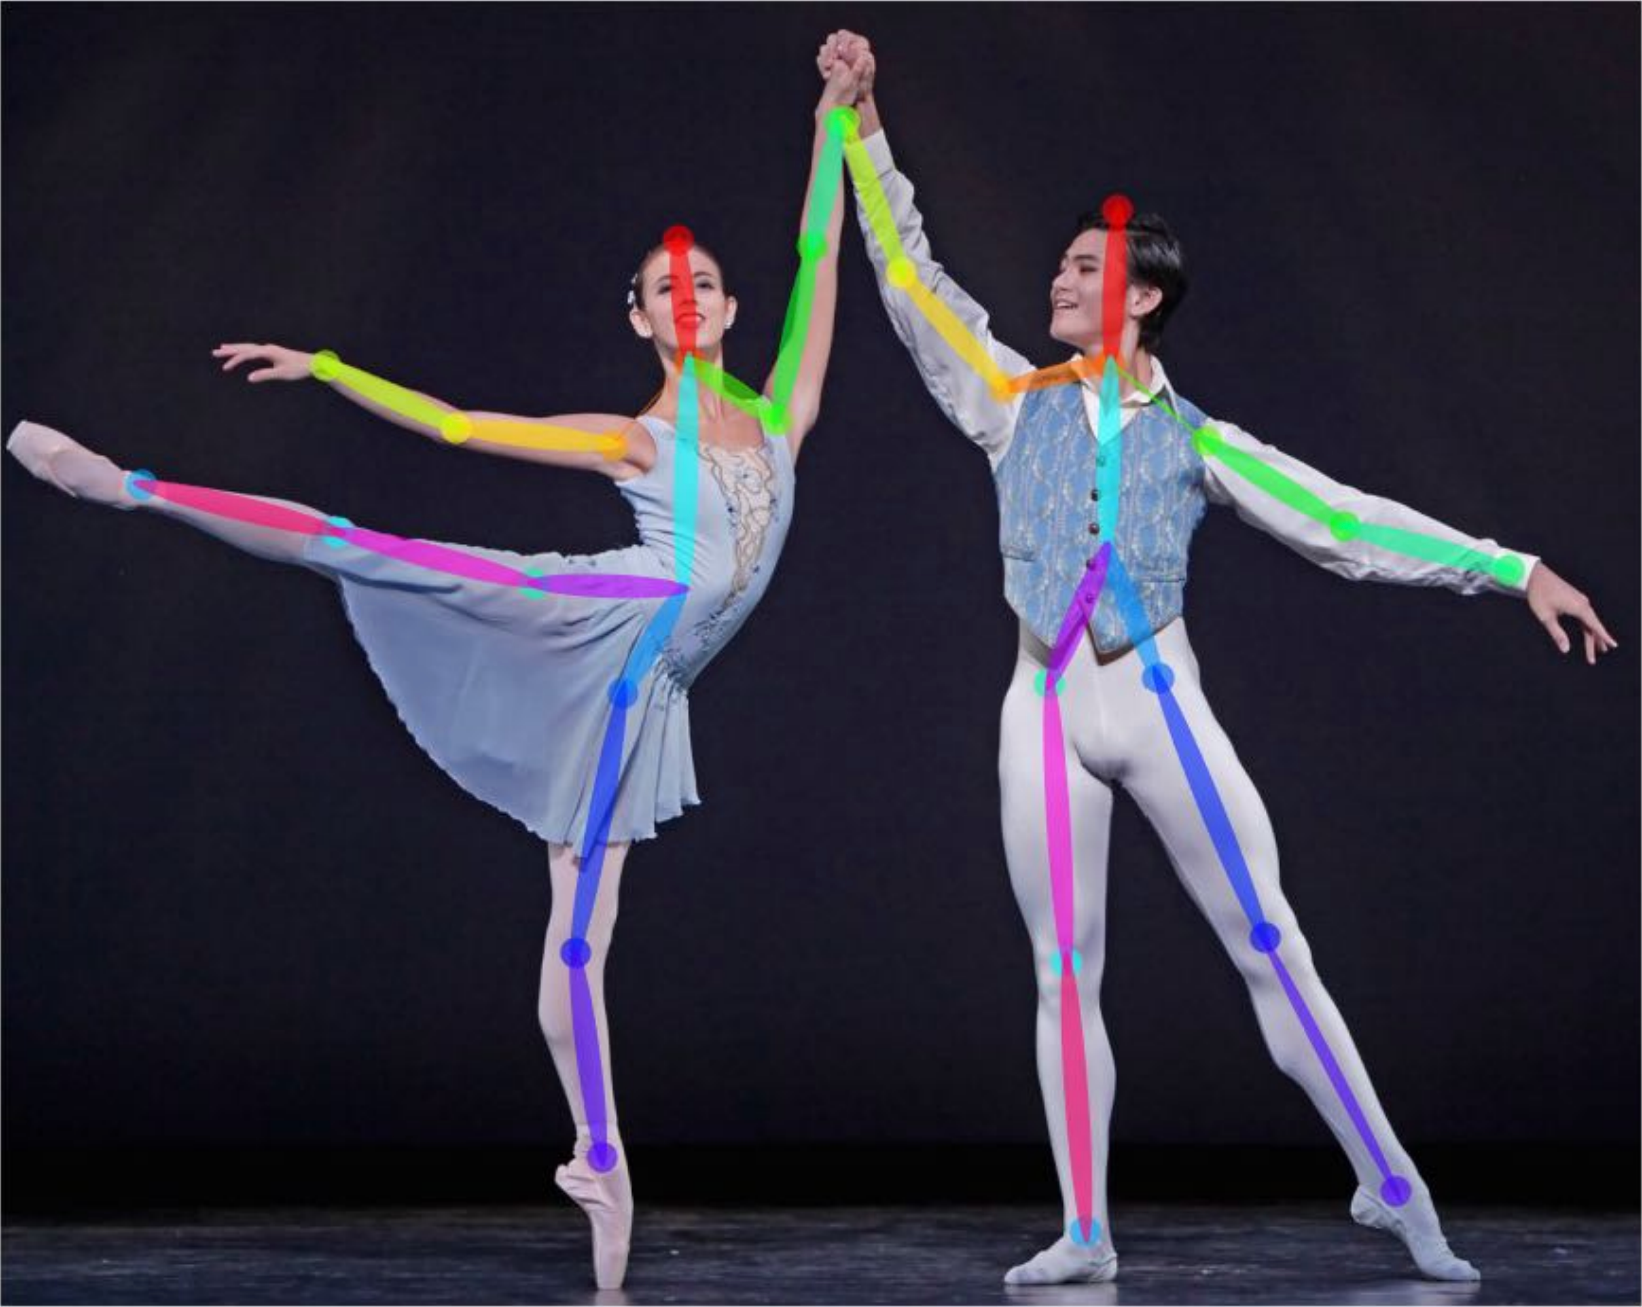
\includegraphics[width=0.9\linewidth]{img/openpose_pipeline_e}
    \label{fig:oppE}
    \caption{Parsing Results}
  \end{subfigure}
  \caption{The pipeline described in \cite{cao2017realtime}. The input image \ref{fig:oppA} is fed into the two networks which produce joint detections in confidence maps \ref{fig:oppB} and \gls{paf}s \ref{fig:oppC}. They then preform bipartite matching in \ref{fig:oppD} to determine which detected joints should be connected by a limb. \ref{fig:oppE} shows the finished results.}
\end{figure}

Using the method described in \cite{cao2017realtime} we however don't get any information if some pairs of joints are missing, leading to an incomplete skeleton. 


A lot of research\footnote{TODO: Cite Research} has been going into extracting human pose either from RGB images, or using depth images. Although many methods exists such as \emph{Histogram of Gradients (HoG)} classifiers,

A lot of research has been done in estimating human pose in two dimensions, as this is where we have quite large datasets, such as the MPII, or the Human 3.6M datasets \cite{andriluka14cvpr,h36m_pami}.

\textbf{Background extraction}

\textbf{HoG classifiers}


\textbf{Motivation for 3D pose} To train any network using supervised learning, we need large amounts of training data. One of the goals for the MECS project is to do \emph{Human Activity Recognition (HAR)}, so one can track the user from day to day and look for patterns that could lead to worsening living conditions. We also want to be able to recognize the activity from any viewpoint, and this is where a 2D approach will lack robustness. This is because any HAR model trained solely on 2D data, will only be able to recognize the activity from the views it has seen the activity being preformed. A 3D approach will provide us with robustness in respect to view-independentness.


